
\chapter{Демонстрация работы программы решения теоретико-графовой
  задачи в семантической памяти}
\label{cha:AlgoDemo}

\section{Задание}
\label{sec:AlgoDemo_task}

На этом этапе выполнения расчетной работы вам необходимо будет
продемонстрировать пошаговое выполнение алгоритма в sc-памяти. Сам
алгоритм и структуры данных для него вы уже исследовали на предыдущих
этапах расчетной работы, а сейчас надо будет продемонстрировать
графодинамику выполнения алгоритма. Это значит, что вся информация,
необходимая для работы вашего алгоритма, должна храниться в sc-памяти
и там же и обрабатываться. В качестве примера <<неудобства>>, которое
вам может принести такое требование, я могу привести невозможность
использования привычной матрицы смежности/инцидентности.  Поэтому для
прохождения этого этапа вам придется взглянуть на алгоритм, решающий
выбранную задачу, под другим углом.

\section{Волновой алгоритм поиска одного из минимальных путей в
  неориентированном графе}
\label{sec:AlgoDemo_algo}

\subsection{Описание алгоритма}
\label{sec:AlgoDemo_algo_desc}

Алгоритм поиска одного из минимальных путей в неориентированном графе
является волновым и основан на понятии волны. В рамках этого алгоритма
волной называется множество вершин, каждая из которых является в
обрабатываемом графе смежной хотя бы одной вершине из предыдущей
волны. Волна, для которой нет предыдущей волны, называется начальной и
состоит из вершины, от которой начинается поиск минимального
пути. Волна, включающая конечную вершину пути, называется
конечной. Таким образом, наш алгоритм можно задать следующим перечнем
шагов:

\begin{enumerate}
\item Добавить все вершины графа, кроме начальной вершины пути, во
  множество непроверенных вершин.
\item Создать новую волну и добавить в нее начальную вершину пути.
\item Начальная волна – это новая волна. Новой волной будем называть
  последнюю созданную волну.
\item Сформировать следующую волну для новой волны. В нее попадет та
  вершина, которая является смежной вершине из новой волны и
  присутствует во множестве непроверенных вершин. Если вершина попала
  в формируемую волну, то ее надо исключить из множества непроверенных
  вершин. Созданную волну установить как следующую для новой волны, и
  после этого созданную волну считать новой волной.
\item Если новая волна пуста, то между вершинами не существует
  пути. Завершить алгоритм.
\item Если в текущей волне есть конечная вершина, то перейти к пункту
  7, иначе к пункту 4.
\item Сформировать один из минимальных путей, проходя в обратном
  порядке по списку волн. Завершить алгоритм.
\end{enumerate}

\subsection{Пример выполнения алгоритма в sc-памяти}
\label{sec:AlgoDemo_example}

\subsubsection{Соглашения по демонстрации}
\label{sec:AlgoDemo_demo_conv}

Перед демонстрацией выполнения алгоритма в sc-памяти нам необходимо
установить некоторые соглашения по формирование SCg-рисунков.

При записи графов я буду использовать сокращенную форму - атрибуты для
вершин и связок не приводятся, однако вы должны помнить, что
сокращенная форма используется только для наглядности.

В качестве программных переменных, которые используются в ходе работы
алгоритма, я буду использовать sc-переменные. Для указания значения
sc-переменной используется отношение \rel{значение}.  На рисунке 3.1
задано значение для sc-переменной \vidtf{beg\_vertex}.

\begin{figure}[h!]
  \centering
  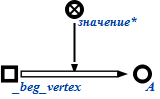
\includegraphics{3/Value_sc_var}
  \caption{Пример указания значения sc-переменной \vidtf{beg\_vertex}}
  \label{fig:Value_sc_var}
\end{figure}

Однако я буду сокращать способ, показанный на
рис.~\ref{fig:Value_sc_var}, опуская знак отношения
\rel{значение}. Таким образом, будет использована форма, показанная на
рис.~\ref{fig:Short_value_sc_var}. Имейте в виду, что полученная
sc-конструкция не является корректной в семантическом смысле, но в
данном разделе использование именно такой формы позволит сделать
рисунки более понятными.

\begin{figure}[h!]
  \centering
  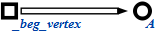
\includegraphics{3/Short_value_sc_var}
  \caption{Пример сокращенного указания значения sc-переменной
    \vidtf{beg\_vertex}}
  \label{fig:Short_value_sc_var}
\end{figure}

Последнее, о чем мы договоримся, будет использование цветов с целью
явного выделения изменений, произошедших с sc-конструкцией. Для этого
я буду использовать следующий перечень цветов:

\begin{itemize}
\item \textcolor{magenta}{фиолетовым} цветом будут выделяться sc-переменные, значение
  которых изменилось;
\item \textcolor{green}{зеленым} цветом будут выделяться созданные sc-элементы;
\item \textcolor{blue}{синим} цветом будут выделяться измененные sc-элементы (например,
  sc-множества, в которые был включен или из которых был исключен
  элемент).
\end{itemize}

Пришло время посмотреть, как же работает наш алгоритм в sc-памяти.

\subsubsection{Демонстрация алгоритма}
\label{sec:AlgoDemo_demo}

Выполнение алгоритма я продемонстрирую через состояния sc-памяти на
каждом элементарном этапе решения задачи. Для всех элементарных
этапов, для которых это возможно, в конце их краткого описания в
скобках будет указан соответствующий номер шага алгоритма из
раздела~\ref{sec:AlgoDemo_algo_desc}.

\newenvironment{algostep}[3]
{
  \newpage
  \label{astep:#2}
  \item \emph{\textbf{#1}}
  
  \begin{figure}[h!]
    \centering
    \includegraphics[scale=#3]{3/#2}
  \end{figure}
}
{
}

\begin{itemize}
\begin{algostep}{Задание входного графа, начальной и конечной вершины
    пути для работы алгоритма}{S1_Input_graph}{0.8}
  
  Переменные изменятся следующим образом:

  \begin{itemize}
  \item \vidtf{graph} получит в качестве значения sc-узел
    неориентированного графа;
  \item \vidtf{beg\_vertex} получит в качестве
    значения вершину А, которая будет начальной для поиска минимального
    пути;
  \item \vidtf{end\_vertex} получит в качестве значение вершину $F$,
    которая будет конечной для поиска минимального пути.  Таким образом,
    из состояния sc-памяти на этом шаге вам должно быть ясно, что будет
    производиться поиск минимального пути между вершинами $A$ и $F$.
  \end{itemize}
\end{algostep}


\begin{algostep}{Создание множества непроверенных вершин (Шаг
    1)}{S2_Create_unchecked_vertexes_set}{0.8}

  Переменная \vidtf{not\_checked\_vertexes} получит в качестве значения
  множество непроверенных вершин обрабатываемого графа (в это множество
  не включена начальная вершина пути $A$).
\end{algostep}


\begin{algostep}{Создание волны, включающей начальную вершину A (Шаги
    2, 3)}{S3_Create_1st_wave}{0.8}

  На этом этапе программа создает первую волну из списка волн. Первая
  волна содержит только начальную вершину пути $A$. Переменная
  \vidtf{new\_wave} получает в качестве значения созданную волну, и в
  будущем будет всегда указывать на вновь созданную волну.

  Переменная \vidtf{waves\_list\_head} указывает на начальный элемент
  списка волн, а переменная \vidtf{waves\_list\_tail} сейчас и в
  последующих шагах – на концевой элемент списка волн.
\end{algostep}


\begin{algostep}{Создание волны, включающей вершины B и С (Шаг
    4)}{S4_Create_next_wave}{0.8}
  
  Для вершин из предыдущей волны являются смежными и входящими во
  множество проверенных вершин только вершины $B$ и $С$. Из них
  формируем новую волну. Обратите внимание на то, что эти вершины
  исключаются из множества непроверенных вершин (см. значение
  переменной \vidtf{not\_checked\_vertexes}).

  Переменная \vidtf{waves\_list\_tail} получает в качестве значения
  созданный элемент списка, а переменная \vidtf{new\_wave} – созданную
  волну.
\end{algostep}


\begin{algostep}{Создание волны, включающей вершину D (Шаг
    4)}{S5_Create_next_wave}{0.8}

  Для вершин из предыдущей волны является смежной и входящей во
  множество проверенных вершин только вершина $D$. Из нее формируем
  новую волну. Обратите внимание на то, что эта вершина исключается из
  множества непроверенных вершин (см. значение переменной
  \vidtf{not\_checked\_vertexes}).

  Переменная \vidtf{waves\_list\_tail} получает в качестве значения
  созданный элемент списка, а переменная \vidtf{new\_wave} – созданную
  волну.
\end{algostep}


\begin{algostep}{Создание волны, включающей вершину F (Шаги 4, 5,
    6)}{S6_Create_last_wave}{0.8}

  Для вершины из предыдущей волны является смежной и входящей во
  множество проверенных вершин только вершина $F$. Из нее формируем
  новую волну. Обратите внимание на то, что эта вершина исключается из
  множества непроверенных вершин (см. значение переменной
  \vidtf{not\_checked\_vertexes}).

  Переменная \vidtf{waves\_list\_tail} получает в качестве значения
  созданный элемент списка, а переменная \vidtf{new\_wave} – созданную
  волну.

  Так как эта волна содержит конечную вершину пути $F$, то на
  следующих этапах мы перейдем к генерации одного из найденных
  минимальных путей.
\end{algostep}


\begin{algostep}{Удаление множества непроверенных
    вершин}{S7_Erase_unchecked_vertexes_set}{0.8}
 
  Подчистим память, удалив множество непроверенных вершин (значение
  переменной \vidtf{not\_checked\_vertexes}), так как оно нам уже не
  надо.
\end{algostep}


\begin{algostep}{Создание связки отношения \rel{путь} (Шаг
    8)}{S8_Create_route_tuple}{0.7}
 
  Начинаем генерацию одного из найденных минимальных путей.

  Создадим связку отношения \rel{путь} и установим ее в качестве
  значения переменной \vidtf{route}. Переменная \vidtf{route\_struct}
  получит в качестве значения ориентированный граф структуры пути, а
  переменная \vidtf{route\_visit} – отношения посещения.
\end{algostep}


\begin{algostep}{Добавление в структуру пути посещения конечной
    вершины генерируемого пути (Шаг
    8)}{S9_Add_end_vertex_visit_to_route_tuple}{0.7}
 
  Добавим в структуру генерируемого пути посещение конечной вершины
  $F$. Созданное посещение получит в качестве значения переменная
  \vidtf{end\_vertex\_visit}.
\end{algostep}


\begin{algostep}{Установка переменных для 1-ой итерации цикла генерации
    структуры пути (Шаг 8)}{S10_Step_building_route_structure}{0.7}
  
  Структура пути строится, начиная с конечной вершины пути $F$.

  На этом этапе переменная \vidtf{curr\_vertex} получит в качестве
  значения текущую обрабатываемую вершину, переменная \vidtf{list\_it}
  – текущий обрабатываемый элемент списка волн, переменная
  \vidtf{curr\_wave} – текущую обрабатываемую волну.
\end{algostep}


\begin{algostep}{Создание посещения вершины на 1-ой итерации цикла
    генерации структуры пути (Шаг
    8)}{S11_Step_building_route_structure_add_visits}{0.7}
 
  Создадим посещение для одной из вершин из волны \vidtf{curr\_wave},
  которая является смежной вершине из переменной
  \vidtf{curr\_vertex}. Для связывающего их ребра тоже создадим
  посещение.
\end{algostep}  


\begin{algostep}{Переход ко 2-ой итерации цикла генерации структуры
    пути (Шаг 8)}{S12_Step_building_route_structure}{0.7}
 
  На этом этапе переменная \vidtf{curr\_vertex} получит в качестве
  значения вершину, для которой было создано посещение на предыдущей
  итерации. Переменная \vidtf{list\_it} – предшествующей элемент
  списка волн для значения переменной \vidtf{curr\_wave} на предыдущем
  этапе. Переменная \vidtf{curr\_wave} – обрабатываемую волну для
  элемента списка из установленного значения \vidtf{list\_it}.
\end{algostep}


\begin{algostep}{Создание посещения вершины на 2-ой итерации цикла
    генерации структуры пути (Шаг
    8)}{S13_Step_building_route_structure_add_visits}{0.7}

  Создадим посещение для одной из вершин из волны \vidtf{curr\_wave},
  которая является смежной вершине из переменной
  \vidtf{curr\_vertex}. На эту роль была выбрана вершина $С$. Для
  ребра, связывающего две вершины, тоже создадим посещение.
\end{algostep}


\begin{algostep}{Переход к 3-ей итерации цикла генерации структуры пути
    (Шаг 8)}{S14_Step_building_route_structure}{0.7}
 
  На этом этапе переменная \vidtf{curr\_vertex} получит в качестве
  значения вершину, для которой было создано посещение на предыдущей
  итерации. Переменная \vidtf{list\_it} – предшествующей элемент
  списка волн для значения переменной \vidtf{curr\_wave} на предыдущем
  этапе. Переменная \vidtf{curr\_wave} – обрабатываемую волну для
  элемента списка из установленного значения \vidtf{list\_it}.
\end{algostep}


\begin{algostep}{Создание посещения вершины на 3-ей итерации цикла
    генерации структуры пути (Шаг
    8)}{S15_Step_building_route_structure_add_visits}{0.7}
 
  Так как для вершины $A$ уже создано посещение, то делать это
  повторно алгоритм не будет. А вот посещение ребра между вершинами
  $A$ и $С$ необходимо создать.

  Структура пути создано, поэтому завершаем цикл и переходим к очистке
  sc-памяти от уже ненужных sc-конструкций.
\end{algostep}

\begin{algostep}{Удаление списка волн}{S16_Erase_waves_list}{0.7}
 
  Удалим список волн. Переменные \vidtf{list\_it},
  \vidtf{waves\_list\_head}, \vidtf{curr\_wave},
  \vidtf{waves\_list\_tail} окажутся без значений.
\end{algostep}


\begin{algostep}{Результат работы алгоритма}{S17_Result}{0.7}
 
  На данном этапе продемонстрирован результат работы алгоритма,
  значение переменной \vidtf{route} будет возвращено в вызывающий
  контекст.
\end{algostep}
\end{itemize}

%%% Local Variables: 
%%% mode: latex
%%% TeX-master: "main"
%%% End: 
